\section{随机对象}
\label{sec:pspace-random-objects}

第~\ref{chap:random-variables}章把随机变量定义为样本空间上的实值函数，并直接对$\{X\in B\}$谈概率。那时事件族是全部子集或者只涉及区间，$\{X\in B\}$是否为事件不成问题。现在事件族是指定的$\mathcal{F}$，一个函数的原像未必落在$\mathcal{F}$里；而我们还会观测向量、矩阵、图这样的对象。什么样的函数才配称为随机变量？

\paragraph{可测性：观测引出的问题都有概率}
回到只知道点数和的观察者，他的事件族是$\sigma(S)$。若他想研究第一枚骰子的点数$X_1$，就会遇到$\{X_1=1\}\notin\sigma(S)$：这个“随机变量”提出的问题，他的事件族无法回答。所以随机变量的定义必须保证，凡是由它引出的“取值落在某个集合中”的问题，答案都在事件族里。卷四的可测映射正是这个要求。

\begin{definition}[随机对象与随机变量]
\label{def:pspace-random-object}
设$(\Omega,\mathcal{F},\mathbb{P})$是概率空间，$(E,\mathcal{E})$是可测空间。映射$X:\Omega\to E$若满足
\begin{equation}
  X^{-1}(B)=\{\omega\in\Omega:X(\omega)\in B\}\in\mathcal{F},\qquad B\in\mathcal{E},
  \label{eq:pspace-measurable}
\end{equation}
则称$X$为取值于$E$的\term{随机对象}（random element）。取值于$(\mathbb{R},\mathcal{B}(\mathbb{R}))$的随机对象称为随机变量，取值于$(\mathbb{R}^{d},\mathcal{B}(\mathbb{R}^{d}))$的称为$d$维随机向量。
\end{definition}

图~\ref{fig:pspace-random-object-map}画出了这个定义。$X$把$\Omega$中的点送到$E$中；对$E$中的集合$B$，把所有被送进$B$的样本点收集起来，就是原像$X^{-1}(B)$。这个原像可以由几块分开的区域组成，可测性要求它是事件，从而有概率。

\begin{BookInlineFigure}
  \centering
  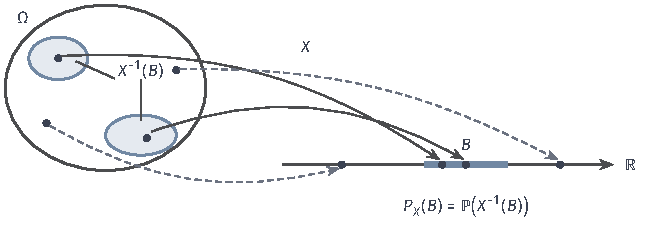
\includegraphics[width=110mm]{figures/07-probability/02-measure-theoretic-probability/tikz/pspace-random-object-map/figure.pdf}
  \caption{随机变量$X:\Omega\to\mathbb{R}$与原像。实线箭头把浅蓝的两块区域中的点送进集合$B$（粗蓝线段），虚线箭头把其他点送到$B$之外。$X^{-1}(B)$是两块区域之并，可测性要求它是事件，它的概率就是取值落在$B$中的概率。}
  \label{fig:pspace-random-object-map}
\end{BookInlineFigure}

定义要求对$\mathcal{E}$中\emph{每个}集合检查原像，实际操作时只需检查一个生成族。卷四的生成族判据说：若$\mathcal{E}=\sigma(\mathcal{C})$，则$X$可测当且仅当对每个$C\in\mathcal{C}$都有$X^{-1}(C)\in\mathcal{F}$。原因是原像运算与补集、可数并交换，使得原像为事件的集合$B$构成一个$\sigma$代数，它包含$\mathcal{C}$，也就包含$\sigma(\mathcal{C})$。对实值函数，取半直线为生成族，得到常用的判别：
\begin{equation}
  X\text{ 是随机变量}\iff\{X\leq x\}\in\mathcal{F}\quad\text{对一切 }x\in\mathbb{R}.
  \label{eq:pspace-rv-criterion}
\end{equation}

\paragraph{常见的取值空间}
映射$\bm{X}=(X_1,\dots,X_d):\Omega\to\mathbb{R}^{d}$是随机向量，当且仅当每个坐标$X_i$都是随机变量。一方面，坐标投影连续，因而Borel可测，可测映射的复合仍可测。另一方面，$\mathcal{B}(\mathbb{R}^{d})$由左下象限生成，而
\[
  \{\bm{X}\in(-\infty,x_1]\times\cdots\times(-\infty,x_d]\}=\bigcap_{i=1}^{d}\{X_i\leq x_i\}
\]
是$d$个事件之交。所以第~\ref{chap:random-vectors}章逐个坐标定义的随机向量，正好是这里的$\mathbb{R}^{d}$值随机对象。

随机矩阵可以看成拉直的向量。把$m\times n$实矩阵按元素排成$\mathbb{R}^{mn}$中的向量，$\mathbb{R}^{m\times n}$就带有Borel $\sigma$代数，随机矩阵$\bm{M}$可测当且仅当每个元素$M_{i,j}$都是随机变量。例如随机向量$\bm{X}$的外积$\bm{X}\bm{X}^{\top}$，其元素$X_iX_j$是随机变量的乘积，所以它是随机矩阵。

有限集合是另一类常见的取值空间，配上全部子集作为事件族。这时可测性只需检查单点：$X$可测当且仅当对每个可能的取值$g$，$\{X=g\}\in\mathcal{F}$，因为任何子集都是有限个单点之并。

\paragraph{有限随机图}
以$3$个带标号顶点上的随机图为例。$3$个顶点之间有$3$条可能的边，每条边出现与否用一个比特记录，样本空间是$\Omega=\{0,1\}^{3}$，取全部子集为事件族，并让$8$个结果等可能。映射$G$把结果$\omega=(e_{1,2},e_{1,3},e_{2,3})$送到边集为$\{\{i,j\}:e_{i,j}=1\}$的图。取值空间$E$是这$3$个顶点上全部$2^{3}=8$个图，同样取全部子集。

在这个模型里$\Omega$与$E$一一对应，可测性不成问题。值得注意的是由图算出的数值。边数$N=e_{1,2}+e_{1,3}+e_{2,3}$是$E$上函数与$G$的复合，它把$8$个图分成$4$组（图~\ref{fig:pspace-random-graph}），由此得到
\[
  \mathbb{P}(N=0)=\tfrac18,\quad \mathbb{P}(N=1)=\tfrac38,\quad \mathbb{P}(N=2)=\tfrac38,\quad \mathbb{P}(N=3)=\tfrac18 .
\]
“图是三角形”是事件$\{N=3\}$，“图连通”是$\{N\geq2\}$，因为$3$个顶点上的图连通当且仅当至少有$2$条边。

\begin{BookInlineFigure}
  \centering
  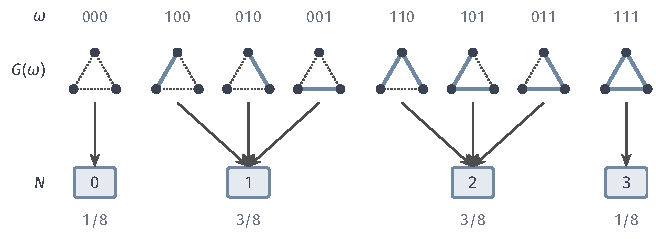
\includegraphics[width=111mm]{figures/07-probability/02-measure-theoretic-probability/tikz/pspace-random-graph/figure.pdf}
  \caption{$3$个顶点上的随机图。上行是结果$\omega=(e_{1,2},e_{1,3},e_{2,3})$，中间是对应的图$G(\omega)$，蓝色实线是出现的边，点线是未出现的边；顶点$1$在上，$2$在左下，$3$在右下。边数$N$把$8$个等可能的图分成$4$组，下方是各组的概率。}
  \label{fig:pspace-random-graph}
\end{BookInlineFigure}

更大的随机图也一样：$n$个顶点有$n(n-1)/2$条可能的边，取值空间有$2^{n(n-1)/2}$个图。边数、三角形个数、最大度数、是否连通，都是有限集合上的函数，与$G$复合后自动成为随机变量。一般地，若$X$是取值于$(E,\mathcal{E})$的随机对象，$g:E\to E'$是可测映射，则对$B\in\mathcal{E}'$，
\[
  (g\circ X)^{-1}(B)=X^{-1}\bigl(g^{-1}(B)\bigr)\in\mathcal{F},
\]
因为$g^{-1}(B)\in\mathcal{E}$。所以$g(X)$也是随机对象。连续函数关于Borel $\sigma$代数可测，于是随机向量的和、积、范数，随机对称矩阵的迹，都是随机变量。

\paragraph{观测生成的事件族}
可测性说明观测\emph{不超出}事件族的回答能力。反过来也可以问：一个观测本身能回答哪些问题？观测$X$之后，对每个$B\in\mathcal{E}$，我们都能判断$X\in B$是否成立，也就是判断事件$X^{-1}(B)$是否发生。这些事件收集起来，就是$X$提供的信息。

\begin{definition}[观测生成的$\sigma$代数]
\label{def:pspace-generated-sigma}
设$X:\Omega\to E$是取值于$(E,\mathcal{E})$的随机对象。称
\begin{equation}
  \sigma(X)=\bigl\{X^{-1}(B):\ B\in\mathcal{E}\bigr\}
  \label{eq:pspace-generated-sigma}
\end{equation}
为$X$\term{生成的$\sigma$代数}（$\sigma$-algebra generated by $X$）。对多个随机对象$X_1,\dots,X_n$，$\sigma(X_1,\dots,X_n)$指向量$(X_1,\dots,X_n)$生成的$\sigma$代数。
\end{definition}

$\sigma(X)$确实是$\sigma$代数：$X^{-1}(E)=\Omega$，并且原像与补集、可数并交换，
\[
  \bigl(X^{-1}(B)\bigr)^{\mathrm{c}}=X^{-1}(B^{\mathrm{c}}),\qquad \bigcup_{k}X^{-1}(B_k)=X^{-1}\Bigl(\bigcup_kB_k\Bigr).
\]
它包含于$\mathcal{F}$，这就是可测性。它也是使$X$可测的最小$\sigma$代数：任何使$X$可测的$\sigma$代数都必须含有全部原像$X^{-1}(B)$。

当$X$只取有限个值时，$\sigma(X)$的原子就是$X$的各个等值集$\{X=x\}$，事件是若干等值集之并。第~\ref{sec:pspace-events}节的“只知道点数和”就是$\sigma(S)$，它的原子是$11$条反对角线；“只知道较大点数”就是$\sigma(M)$，原子是$6$个L形区域。只知道“点数和是否为$7$”，对应的是指示变量$\mathbf{1}_{\{S=7\}}$，它生成的$\sigma$代数只有$4$个事件。

\paragraph{函数只会减少信息}
对观测结果再作变换，信息不会增加。设$g$可测，对$B\in\mathcal{E}'$，
\[
  \bigl(g(X)\bigr)^{-1}(B)=X^{-1}\bigl(g^{-1}(B)\bigr)\in\sigma(X),
\]
所以$\sigma(g(X))\subseteq\sigma(X)$。在骰子的例子里，$\mathbf{1}_{\{S=7\}}$是$S$的函数，$\sigma(\mathbf{1}_{\{S=7\}})\subseteq\sigma(S)$：知道点数和就知道它是否为$7$，反之不行。若$g$是双向可测的一一映射，两个方向都用上述包含关系，得到$\sigma(g(X))=\sigma(X)$：可逆的重新编码不改变信息。

木棍上的随机点给出一串逐渐精细的观测。设$\Omega=[0,1)$，$\omega$的二进制展开为$0.D_1D_2D_3\cdots$，取不以无穷个$1$结尾的那种展开，即
\[
  D_k(\omega)=\lfloor2^{k}\omega\rfloor-2\lfloor2^{k-1}\omega\rfloor\in\{0,1\}.
\]
记$K=\lfloor4\omega\rfloor$，它告诉我们$\omega$落在哪个四分之一区间。图~\ref{fig:pspace-nested-information}列出了几个观测的原子。$D_1=\lfloor K/2\rfloor$与$D_2=K-2D_1$都是$K$的函数，所以$\sigma(D_1)$和$\sigma(D_2)$都包含于$\sigma(K)$；$K$又是$\lfloor8\omega\rfloor$的函数。$\sigma(D_2)$的一个原子是$[1/4,1/2)\cup[3/4,1)$，由两段不相邻的区间组成，它说明粗信息未必是“把区间分得粗一点”。$\sigma(D_1)$与$\sigma(D_2)$互不包含，两者合起来恰好是$\sigma(K)$。

\begin{BookInlineFigure}
  \centering
  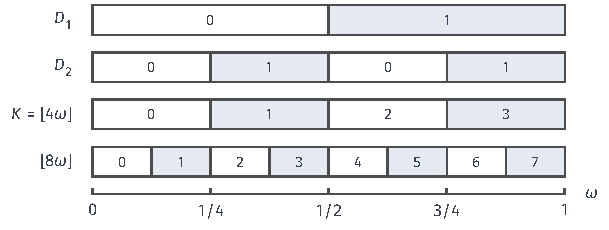
\includegraphics[width=103mm]{figures/07-probability/02-measure-theoretic-probability/tikz/pspace-nested-information/figure.pdf}
  \caption{$\Omega=[0,1)$上几个观测生成的原子。每一行把$[0,1)$分成若干格，格内数字是该观测的取值，浅蓝格子取奇数值。$D_1$、$D_2$是前两位二进制数字，$K=\lfloor4\omega\rfloor$。$\sigma(D_1)$与$\sigma(D_2)$都包含于$\sigma(K)$，$\sigma(K)$又包含于$\sigma(\lfloor8\omega\rfloor)$；$D_2$的原子各由两段不相邻的区间组成。}
  \label{fig:pspace-nested-information}
\end{BookInlineFigure}

观测$X(\omega)=\omega$本身生成全部Borel集，它提供完整的信息。这里讨论的都是一次观测，或同时取得的有限个观测。信息随时间逐步增加、后一时刻知道得比前一时刻多的情形，要用一列递增的$\sigma$代数描述，属于随机过程的内容。第~\ref{chap:conditional-expectation}章将以$\sigma(X)$为“已知信息”，研究给定信息后怎样求平均。
